\title{Exploiting Mobile Entities for Urban Air Quality Monitoring \\ MPP1}
\author{Dale Myers \\ 0942590}
\date{\today}

\documentclass[12pt]{article}

\usepackage{tabularx}
\usepackage{float}
\usepackage{url}
\usepackage{verbatim}
\usepackage{fixltx2e}
\usepackage{graphicx}
\usepackage{parskip}
\usepackage{hyperref}
\usepackage{mhchem}
\usepackage{todonotes}
\usepackage{minted}
\usepackage{upgreek}
\usepackage{comment}
\usepackage{fullpage}
\usepackage{pdflscape}

\newcommand{\mahesh}[1]{\todo[inline,color=green!40]{#1}}
\newcommand{\idea}[1]{\todo[inline,color=blue!40]{#1}}

\begin{document}

\todo[inline]{Orange todo notes are things which I am considering. Please feel free to comment on these.}

\mahesh{Green notes are questions directly for you which I am unsure about.}

\idea{Blue notes are ideas that I have had for later in the project.}


\maketitle
\thispagestyle{empty}
\newpage

\tableofcontents
\thispagestyle{empty}
%\todototoc
%\listoftodos


\newpage

\setcounter{page}{1}

\mahesh{We have been told not to put too much background into these reports, however since I have only done background research I'm not sure how to go about this. I have followed almost exactly the structure that you laid out for me in our last meeting. Is this suitable?}

\section{Introduction}\label{intro}

The aim of the project is to evaluate the suitability of the following model of taking air quality measurements with the goal of providing data quickly, whilst still remaining efficient. 



\section{Preliminary Work}\label{preliminary}


During the course of working on the MPP and MPP1 reports, preliminary work was carried out in order to efficiently form a work plan. In this preliminary work the challenges which would be faced were identified, as well as a background report on the definition of \emph{air quality}, the creation of heat maps, which are the standard representation format for display air quality information \todo{CITE ME}. Finally some research was carried out into building an appropriate sensor platform.


\subsection{Challenge Identification}\label{challenges}

In order to effectively evaluate the task at hand the challenges involved must first be identified. With regards to this the following challenges were identified as being the most important overall aims for the project, at least in the current stage. 

\begin{itemize}
	\item What to measure?

	In order to measure air quality effectively a standard definition should be used. Research showed that there was very little consensus on the definition of air quality and so a definition which this thesis will use as the standard must be defined. The definition must also include a list of chemicals so that the appropriate hardware can be used to generate readings. This ensures that the solution is also cost effective. 

	\item Deployment considerations

	In the MInf Project Proposal stage it was discovered that there are certain considerations which must be made in order to effectively measure air quality. As can be seen in Figure~\ref{fig:stationarypollutantbuildup}, which shows the initial motion of a bus with an air quality sensor on the top deck, pollutants build up when the bus is stationary and only disperse after a certain amount of time which is dependent on the current weather and motion of the bus.

	\begin{figure}[H]
        \begin{center}
                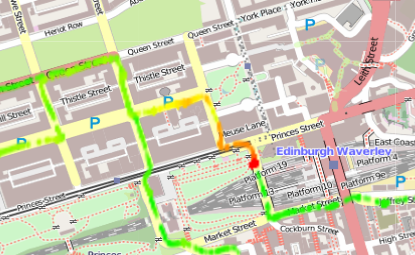
\includegraphics[scale=0.8]{./images/mpp1/StationaryPollutantBuildUp.png} 
                \caption{Example of pollutant build up in stationary situations. In this example the bus starts where the highest concentration of pollutants is found, denoted by the red, and moves in a northern direction initially.}
                \label{fig:stationarypollutantbuildup}
        \end{center}
	\end{figure}

	It was also found that certain measurements were dependant on other factors. Temperature, for instance, was dependant on the direction of the bus due to the sensors location at the back. When the bus turned towards the south, the sunlight hit the temperature sensor directly which caused a spike in temperature readings. Humidity showed a similar response to the air pollutants. 

	With regards to this it has been determined that in order to continue with the original plan of mounting the sensors on buses, a suitable enclosure must be designed which will remove direct sunlight and build up of pollutants from the data. It may be that it is not possible to remove the pollutant build up and stops may need to be recorded so that the data can be corrected for this discrepancy, whether by adjusting the recorded values automatically, or simply removing it from the data set. 

	\item Calibration

	Each sensor is different from other models and even subtly different from other samples of the same model. In order to compensate for this calibration must be performed. In certain situations it may be sufficient to simply measure against a baseline before starting the data collection, however in others calibration may be needed periodically. 

	Projects such as the OpenSense deployment in Zurich~\cite{opensensezurich} perform periodic calibrations when the trams come within a certain distance of each other. 


	\item Data collection
	
	Data collection is the main goal of this project. The aim of this is to have a method which is both efficient, in terms of power consumption and reliability, and responsive. In order to do this there are multiple methods of uploading data which can be trialled to find that which is the most effective.

	\item Interpolating and extrapolation

	When dealing with a data set such as air quality readings where we only have sparse data measurements it is important to represent the data as clearly as possible. In order to do this a method of interpolation, and potentially extrapolation, must be employed. Multiple different models will be evaluated and compared in order to select the model which is most appropriate for generating the expected output.

\end{itemize}



\subsection{Air Quality}\label{airquality}

\subsubsection{Definition}\label{airqualitydefinition}

A definition of air quality is a difficult problem which has not been solved. Many institutions measure and record what they refer to as ``air quality'', however the only thing these measurements have in common is that no two are the same. In order to research the area of ``air quality'' further we must have a concrete definition of what air quality is. Current definitions give a simple definition of ``air quality'' as being antonymous to that of air pollution in that higher air quality is the equivalent to low air pollution\cite{bcaq}. This implies that not only should the metrics used for defining air quality be considered, but also those used to define air pollution.

Looking at statements and measurements by various authorities around the world \cite{epapollutants}\cite{airqualityobjectives}\cite{cleanairnavigation}\cite{naaqs}\cite{whoguidelines}, we can build a list of common pollutants which are measured:


\begin{itemize}
\item Sulphur dioxide
\item Nitrogen dioxide
\item PM10 
\item PM2.5
\end{itemize}

These chemicals can form the basis of pollutants which in turn can help define ``air quality''. By looking at other sources\cite{meaningsofenvironmentalterms},  proposed definition of ``air quality'' is as follows:

\begin{quote}
``The current measurements of the concentrations of certain pollutants in the air relative to the requirements of one or more biotic species or to any human need or purpose.''
\end{quote}

\subsubsection{Measurement}\label{airqualitymeasurement}

\paragraph{Sensors and Calibration} \hspace{0pt} \\

In order to measure pollutants and other factors relating to air quality we rely on electrochemical, solid state, or mechanical sensors, with the former being the most popular. The nature of sensors presents some unique problems. Mechanical sensors, such as those used for measuring pressure, may seize up and provide inaccurate measurements. Electrochemical sensors, which use an active surface, decay over time. This project will be using electrochemical sensors only, and so only suffers from the latter problem. 

\emph{How Electrochemical Sensors Work}

An electrochemical sensor is made up of the following components:\cite{intlelectrochemicalsensor}

\begin{itemize}
	\item Anode
	\item Cathode
	\item Gas Permeable Membrane % - This covers the electrode in the sensor from contamination, while still allowing gases to pass though.
	\item Electrolyte % - Something about reactions...
\end{itemize}

By reacting the target gas at the anode and measuring the resulting current generated we can calculate how much of the target gas is present. In sensors which react with the target gas at the anode, oxygen is needed at the cathode as can be seen from the following chemical reactions.

At anode:

\begin{align*}
	\cee{\emph{Carbon Monoxide: } CO + H_{2}O &-> CO_{2} + 2H+ 2e- \\
	\\
	\emph{Hydrogen Sulphide: } H_{2}S + 4H_{2}O &-> H_{2}SO_{4} + 8H+ + 8e- \\
	\\
	\emph{Nitrous Oxide: } NO + 2H_{2}O &-> HNO_{3} + 3H+ + e- \\
	\\
	\emph{Hydrogen Cyanide: } 2HCN + Au &-> HAu(CN)_{2} + H+ + e-}
\end{align*}
At cathode:
\begin{align*}
	\cee{O_{2} + 4H+ + 4e- &-> 2H_{2}O \\}
\end{align*}

Insufficient oxygen at the cathode causes the cathode to degrade resulting in changing readings. 

In other types of sensors, which react with the target at the cathode, oxygen is not always necessary. For example:

\begin{align*}
	\cee{\emph{Nitrous Oxide: } NO_{2} + 2H+ + 2e- &-> NO + H_{2}O \\
	\\
	\emph{Chlorine: } Cl_{2} + 2H+ + 2e- &->  2HCl\\
	\\
	\emph{Ozone: } O_{3} + 2H+ + 2e- &-> O_{2} + H_{2}O }
\end{align*}

While oxygen is not a requirement, these sensors do eventually degrade due to the fact that no chemical reaction is going to be 100\% efficient.

\emph{Solid State Sensors}

I'm pretty sure the sensors I have are electrochemical so I haven't read much about this yet, but I will have 

\emph{Calibration}

In order to continue using sensors as they degrade, they must be calibrated regularly. The most simple method of calibration, employed by projects such as OpenSense, simply use a known reliable sensor to take readings at the same point of space and time and calibrated using this data as a reference.






\subsection{Heat maps}\label{heatmaps}


\subsubsection{Definition}\label{heatmapdefinition}

A heat map is a two dimensional graphical representation of a matrix using colours to correspond to different magnitudes of values. It is a thematic map of a matrix, although can also be applied to geographical maps. 

\begin{figure}[H]
        \begin{center}
                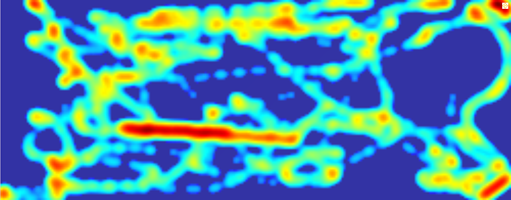
\includegraphics[scale=0.5]{./images/heatmaps/ExampleMouseMove.png}
                \caption{Example heat map generated from mouse movements}
                \label{fig:mousemoveheatmap}
        \end{center}
\end{figure}

Heat maps are generally used to quickly display which values in a matrix have the greatest magnitude and how they compare to surrounding values. Figure~\ref{fig:mousemoveheatmap}, which represents mouse movements on a website clearly shows a horizontal band in the middle which indicates that the users mouse spent a lot of time there. 

\paragraph{Calculations and Colour Progression} \hspace{0pt} \\


In order to create an image representation of the matrix, a colour progression must be chosen. The simplest colour progression method is a hue change on a single colour corresponding to the information. However this may not always be the most suitable method. When giving out information to the public, certain colours tend to represent different things. Red normally has negative connotations while green is the opposite. For this we can use a blended hue colour progression with red at one end of the scale and green at the other.


\paragraph{Representation Matrix} \hspace{0pt} \\

In order to generate the heat map we first need a matrix. A simple matrix can generate an effective heat map as can be seen from the following example.

\begin{figure}[H]
        \begin{center}
                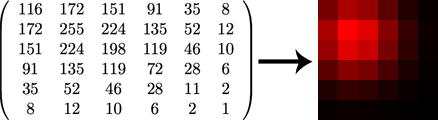
\includegraphics[scale=0.5]{./images/heatmaps/HeatMapGaussianExample.png}
                \caption{Heat Map Generation Example}
                \label{fig:matrixheatmapexample}
        \end{center}
\end{figure}

The example in figure~\ref{fig:matrixheatmapexample} has the maximum value of 255 represented by red (RGB value of \#FF0000) and the minimum value of 1 being almost black (RGB value \#010000). 

\emph{Missing Values}

With many applications there are either missing values in the matrix, or the values cannot be easily placed into a matrix (as is the case for geographical readings). To find the missing values, interpolation of some kind is used. In figure~\ref{fig:matrixheatmapexample} the matrix was generated by placing the value 255 in position (2,2) and performing a Gaussian blur with a filter size of 2 by 2 pixels and sigma equal to 2. 

Irregular data points must be processed further by mapping them onto a matrix. In the case of taking geographical readings, the heat map can be regenerated for each zoom level to ensure the maximum accuracy. 

These methods are not completely accurate and the missing data should be calculated in a manner appropriate to the application.

\subsubsection{Applications in Air Quality Measurement}\label{applicationsinaqmeasurement}

Heat maps are extremely useful to show the concentrations of pollutants in geographical areas. The information is easily given when overlaid on top of a map.  

\begin{figure}[H]
        \begin{center}
                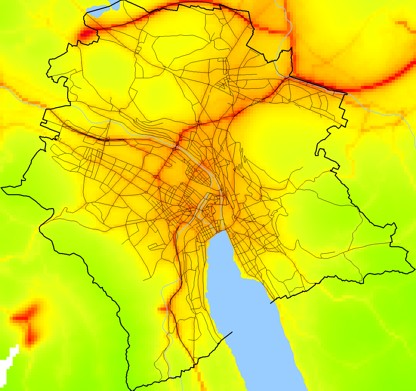
\includegraphics[scale=0.5]{./images/heatmaps/zurichpm.jpg}
                \caption{Particulate matter heat map in Zurich. Source: \url{www.stadt-zuerich.ch}}
                \label{fig:pmheatmapzurich}
        \end{center}
\end{figure}

From the above image we an easily see that the highest concentrations of particulate matter are where the roads are situated indicating a relationship between the two. 






\subsection{Platform Creation}\label{platformcreation}

\subsubsection{Sensor}\label{sensor}

Due to the great expense of using the \emph{Waspmote} platform developed by \emph{Libelium} ~\cite{waspmote}, it was decided that the most suitable option for creating a sensor platform was to use an \emph{Arduino} board of some form. Research showed that it had been used successfully in many hobbyist projects and also in other sensor network research projects. ~\cite{arduinoproj1}~\cite{arduinoproj2}~\cite{arduinoproj3} 

The \emph{Arduino Uno} was selected as a suitably powered, low cost system for the development base. Extra components provided wifi and GPS along with sensors for temperature, humidity, carbon monoxide and ozone. 

Due to a concern about processing power by Dr Marina, a \emph{Raspberry Pi} was also purchased to develop a base sensor from. Should the Uno prove unsuitable the Raspberry Pi will be used. In order to facilitate a faster development time, a conversion shield from Arduino Uno to Raspberry Pi was also purchased. This allows the physical set up of the sensors to stay constant between the two systems. The \emph{arduPi} library ~\cite{ardupi} created by Libelium also allows the software created for the Uno to run on the Pi. A further advantage is that as each sensor has different characteristics and normally requires the implementation of a complex formula, this single implementation ensures that bugs and time spent will be kept to a minimum. 

As the sensor will be subject to a wide variety of weather conditions, a suitable enclosure must be found. This enclosure should protect the electronic components while still allowing readings to be taken. There should also be the ability to provide power to the sensor somehow. This enclosure has not yet been decided on as it is dependent on where and how the sensor will be mounted. 

Currently the components have not yet been delivered and therefore the sensor has not been implemented. 

\subsubsection{Data Collection Framework}\label{datacollectionframework}

In January of this year, preliminary readings were taken with a sensor designed and developed last year by Eric Shane Staples.~\cite{envisensor} This preliminary work was designed as a test for multiple concepts. One of these was a stable data recording and uploading protocol. The sensor would take readings and send them to the receiver over bluetooth which would attempt to upload directly to a server by performing a GET request containing the data to a server. If this failed for whatever reason, or the application detected that there was no internet connection before attempting this, the data would be cached to be uploaded at a later date. The trial was not very demanding but showed that the concept worked in principle. The system can easily be scaled to deal with much more data being returned from any upload points. 

The second part to the framework is the data visualisation ability. The work into heat maps and interpolation models will allow the data to be viewed in simple graphical formats, while still retaining more complex charts and tables. After discussion with Dr Mark Wright, an expert in human-computer interaction, he has agreed to provide his expertise in designing an easy to use, clear interface should it be required. 



\subsection{Conclusion}\label{preliminaryconclusion}

\begin{comment}
Conclusion is finding the right approach to deployment and what sort of gases should I measure and the platform I should use (how can I engineer a platform based on this device)
\end{comment}

\todo[inline]{Do I need a conclusion?}

\section{Calibration}\label{calibration}



* Discuss state of the art
* Identify an approach to use and implement in project (mainly a question of considering different schemes and talking about their effectiveness)

\section{Data Collection}\label{datacollection}

There are many advantages of air quality monitoring, some of which require the latency between taking a reading and it being publicly available to be as small as possible. In order to make this happen two different mechanisms can be employed. 

The first is compression of the data. This can be achieved simply by only taking measurements after a certain time has passed, or the sensor has moved by a specified amount, or both. However, with the knowledge that the data set will be sparse, compressive sampling can be performed which will allow the entire data set to be reconstructed from key readings with minimal loss of information. 

The second method is the rapid upload of data. For this to happen, the data needs to reach an access point as quickly as possible. Opportunistic uploading allows this to happen by moving data from one sensor to another in order to reach an access point rather than relying solely on the original sensor moving into range. 

\subsection{Compressive Sampling}\label{compressivesampling} 

\todo[inline]{The general principle is that you can chose your sample points in order to leave you with a system of linear equations which need to be solved for any given data point. The number of unknowns is greater than the number of equations and normally this gives you infinite possible solutions. By specifying that the solution must also be sparse somehow you can reconstruct the original data (or close enough). JPEG compression works on this principle. It shows that data sampling isn't dependent on the Nyquist Rate as originally thought.}


\subsection{Opportunistic Uploading}\label{opportunisticuploading}

Opportunistic uploading allows a sensor, \emph{B}, to pretend to be an access point so that a sensor with data which needs to be uploaded, \emph{A}, can transfer it's data to \emph{B}. This is an advantage in that if \emph{B} meets an actual access point before \emph{A} does, the data will be transferred with less latency than it would by only using actual access points. 

\begin{figure}[H]
    \begin{center}
        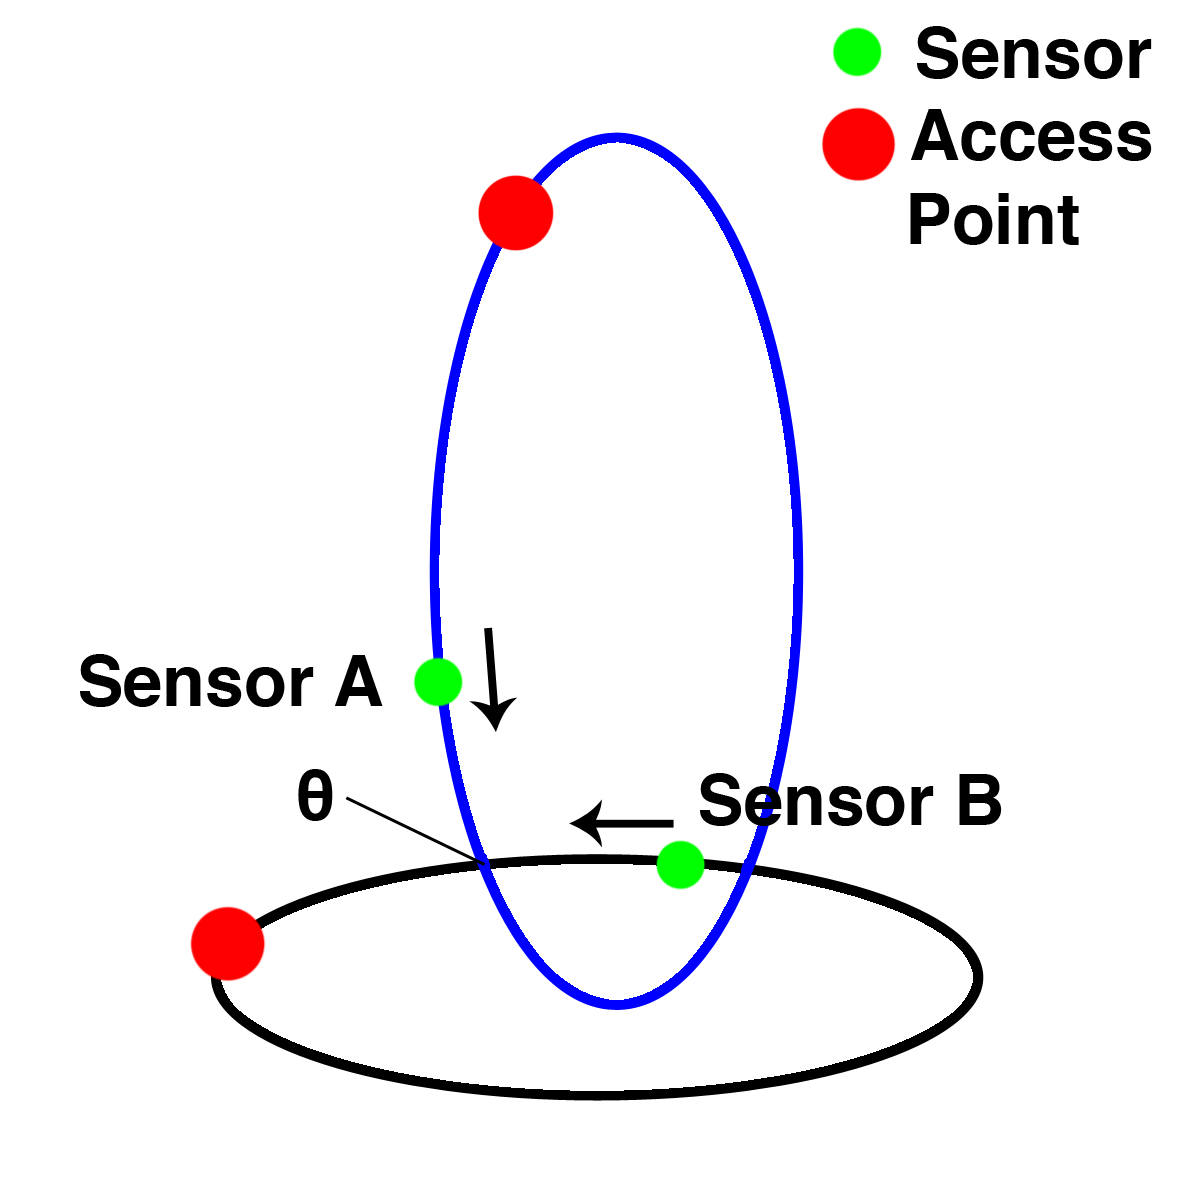
\includegraphics[scale=0.2]{./images/mpp1/Intersection.png}
        \caption{Diagram showing reduced latency. The black arrows indicated the direction of travel of the sensors. $\theta$ is the intersection point of the two routes. It can be seen that sensor A has a much further distance to travel to an access point than sensor B does.}
        \label{fig:opportunisticdiagram}
    \end{center}
\end{figure}

The situation is extremely similar to a routing protocol used in computer networks. The task is to get the information from the sensor to an access point as quickly as possible. Each link will have a certain weight associated with it and it is up to the nodes to select the appropriate route. 

Due to the predictable nature of buses, each node is capable of calculating the time it will take before it comes into range of an access point or other bus, and based on previous encounters, how long this encounter will be and therefore how much data it can upload. All this information can be used to calculate a link ``weighting'' which can be used in any standard routing protocol. 

In the case of this project the task can be simplified greatly by restricting the use of multiple hops so that data can at most move from the original sensor, to a different sensor, to the access point. This allows a single calculation to be performed to decide if data should be uploaded from \emph{A} to \emph{B}. 

There are further considerations which thought has been given to, but most require experimental results in order to answer. 

\begin{itemize}
	\item How much data should be uploaded?

		This is dependent on the upload rate of the data to the new sensor, the upload rate from the new sensor to the access point and the buffer size on the new sensor. 

	\item Which data should be uploaded?

		Older data is getting stale and applications may be waiting on it, however, it may be advantageous to provide the new data as quickly as possible as there may be time sensitive applications which do not require all data. 

	\item How often should we look for other nodes or an access point?

		If we only have access to a single wireless radio, the time a sensor spend scanning for other nodes means it spend less time listening for nodes trying to connect to it. The only solution may be to have two wireless radios. In the case of looking for the access point, this can be done by calculating the distance between the sensor and the access point using GPS data. If the distance is within a specified maximum then the sensor can start trying to connect to the access point. 

	\item Which wireless protocol is the most suitable to use for upload to the access point?

		Wifi is ubiquitous throughout the city and has high transfer rates, however it has a slow handshake. This may be crippling when sensors are only in range of each other for a few seconds at most. Bluetooth or ZigBee have much faster handshakes, but lower throughputs. This would also require dedicated access points across the city rather than simply using open access points or eduroam access points.

	\item Which wireless protocol is the most suitable to use for inter-sensor communication?

		If multiple radios are used then there is a similar situation to the above. 

\end{itemize}

\todo[inline]{I've already answered some of the above questions. Need to be tied together a little bit I think}

Further experimentation is required with hardware to determine the average handshake length, and the average volume of data which is transferred at different relative velocities. This data can then be used to populate the parameters in the algorithm used. 

\todo[inline]{This section needs to be rounded off better}







\section{Geostatistical Mapping}\label{geostatistics}

\mahesh{This was originally laid out differently, but it turns out that all the models are just different types of geostatistical mapping.}

%http://systems.cs.colorado.edu/~caleb/dyspan2012.pdf

When measuring air quality values are only generally generated at points where sensors can easily be placed. With this project we are limited to roads, and indeed where the data collection algorithms have deemed it necessary to collect data. In order to effectively map air pollution a method of calculating the missing values must be found.

Geostatistics is a specific type of statistics which focuses on spatial data. One of the main uses being the prediction of values from a sample set, this being known as \emph{spatial prediction} or \emph{spatial interpolation}~\cite{practicalguidestatisticalmapping}. Within geostatistical mapping there is the ability to use many different interpolation algorithms. Indeed, \emph{A Practical Guide to Geostatistical Mapping of Environmental Variables} by Tomislav Hengl provides a list of just some of the available algorithms: 

\emph{``Inverse Distance, Kriging, Minimum Curvature, Polynomial Regression, Triangulation, Nearest Neighbour, Shepard’s Method, Radial Basis Functions, Natural Neighbour, Moving Average, Local Polynomial, etc.''}

When using this technique we must choose between a mechanical model and a statistical model. A mechanical model is suitable for the cases where no information about the data is available (e.g. range, deviation, mean, etc.). Statistical models use probability theory to estimate the new values using a provided rule set and can therefore be more accurate. 

Different types of each model will be looked at and compared in order to select the most suitable candidate for this project. However, the selection is dependent on factors such as the dataset it's self. This may mean that an accurate selection of model cannot be made until the data collection phase is complete~\cite{mappingairpollutionusinggis}. 

\subsection{Mechanical Models}\label{mechanicalmodels}

\subsubsection{Inverse Distance Weighting}\label{inverseweight}
%http://www.alyrica.net/wifi_mapping

The key component of inverse distance weighting (IDW) is the calculation of new parameters as the weighted average of neighbouring parameters. The weight in this algorithm is calculated as the inverse of the distance from the current point to it's neighbours. The weighting is normalised so that the total of all weights to neighbours is equal to one. This causes the algorithm to slow down with large data sets and so a restriction on search radius may be put in place. 

\todo[inline]{Insert image similar to http://help.arcgis.com/en/arcgisdesktop/10.0/help/0031/GUID-EA2E0EEF-D84E-4856-963E-73AB99DBE58B-web.gif}

\subsubsection{Regression on Coordinates}\label{regressiononcoordinates}

This model assumes that the value at any given point can be calculated using a function which also passes through, or goes close to, all other points. In this case of our three dimensional data (latitude, longitude and value) the function is the equation of a surface. Regression on coordinates does not use any information about the variance of the data. 

\subsection{Statistical Models}\label{statisticalmodels}

Many statistical models require no deliberate correlation between the measurements. Due to the fact that our measurements are taken along bus routes there is a definite correlation of geographic and temporal location information and therefore these models cannot be used. The main remaining model is kriging.

\subsubsection{Kriging}

\idea{Use hue interpolation for the variable and saturation for the variance?}

Kriging is similar to IDW in that it follows the idea that an known point is the weighted average of it's neighbours. It is however more advanced in that it analyses the spatial structure of the data before any calculations take place~\cite{geostatisticalradiomapping}. It also takes into account environmental factors. This allows more accurate predictions. An example of how environmental factors are taken into account is when temperature is measured. IDW provides an answer based on nearby data. Kriging on the other hand would look at factors such as weather patterns, whether there are large bodies of water nearby, elevation, time of year, etc. All this data together allows kriging to be much more effective than simple IDW, however has the disadvantage that these environmental factors also need to be collected. There are 3 main types of kriging:

\begin{itemize}
	\item Ordinary kriging

		Ordinary kriging requires the construction of a variogram~\cite{ordinarykriging}. A variogram is a function which describes the degree of dependence of a spatial field as a function of distance and consists of two parts: an experimental variogram and a model variogram. The experimental variogram is calculated as the variance of each point in the data set plotted against the distance between the two. The model variogram is a simple mathematical function which models the trend of the experimental variogram. Examples of this can be seen in figure~\ref{fig:ordinarykrigingexample}.

		\begin{figure}[H]
        	\begin{center}
                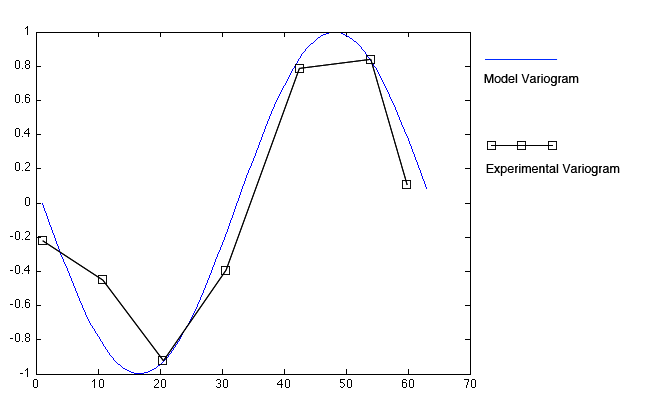
\includegraphics[scale=0.75]{./images/mpp1/KrigingModelFunction.png}
                \caption{Example experimental and model variograms}
                \label{fig:ordinarykrigingexample}
        	\end{center}
		\end{figure}

		When using kriging, as estimate of the variance is also returned with the interpolated results.

	\item Simple kriging

		Simple kriging is similar to ordinary kriging but it does not have the constraint that the weights surrounding a point must add up to one. This produces a less accurate but smoother result. ~\cite{simplekriging}

	\item Universal kriging

		Universal kriging assumes a stationary data set~\cite{universalkriging} and a polynomial trend model. The local trend implemented as part of this model provides some of the most accurate results

	\item Regression kriging

		Regression kriging is universal kriging but uses simple kriging to calculate the interpolated values of the environmental parameters provided to the algorithm ~\cite{regressionkriging}. 
		\mahesh{Land Use Regressions seems to be similar to RK but I cannot find anything which explicitly states what it is.}

\end{itemize}



\subsection{Comparison}\label{interpolationcomparison}

Each model has advantages and disadvantages. Both have lots of exposure to these types of environmental problems. 

In general the mechanical models are easier to implement, require less data and are faster. They have the downside that they are generally much more inaccurate. 

Statistical models are much more difficult to implement and take longer to run. They also require much more data about the environment in order to be as accurate as possible. This data varies and is dependent on what is being measured. In this case we would need information such as road layout, traffic density, building locations and heights, altitude, etc. Generally when being used in similar projects, the calculations are done by software such as \emph{ArcGIS}~\cite{arcgis}, which is unsuitable for this project due to the high cost of \$2500. Free alternatives exist for GIS software but only one of these has the ability to perform kriging. 

With the complexity in mind it would take longer than the project time frame to implement these statistical models. The extra information required would also provide extra difficulty, requiring either a third party data source or extra hardware. It would also be extremely difficult to validate the results. 

The choice is therefore to use a mechanical model. IDW is the simplest and is therefore the choice. Time permitting, the regression on coordinates model will be implemented and compared in order to find which is most suitable. 






\section{Workplan}\label{workplan}

\subsection{MPP Workplan Differences}

\begin{itemize}

\item Create Visualisation Website

	This was moved to the summer due to the fact that it was unnecessary at earlier stages. 

\item Create Base Station \& Add power meter to sensor

	Due to the project changing scope, it was unclear what the physical set up of the sensor would be and so any work on the sensor or anything it interfaced with had to be postponed. 

\item Investigate fountain codes
	
	Again with the project changing scope this was not necessary. 

\item All implementation

	None of this was possible due to the project change. 

\end{itemize}



\subsection{Expert Advice}\label{expertadvie}

Over the last few months contact has been made with various experts in their fields which are related to this project. These people are as follows:

\begin{itemize}

\item Dr Mark Wright

Involved with a group which is working on a very similar project, Dr Mark Wright is an extremely helpful source of information about how to solve implementation problems. His groups goals are slightly different in that they are interested in making this data available, however, with their partnership with Lothian Buses and the time scale they are aiming for, I am hopeful that we can work together to achieve both of our goals. 

\item Dr John Moncrieff 

A professor of Micrometeorology at the \emph{University of Edinburgh}, Dr John Moncrieff, has a research interest in gas diffusion modelling in the earth's atmosphere. With his guidance I am developing a key insight into the optimal model to use to interpolate the sparse data sets generated. 

\item Dr Stuart Sneddon

As the business manager at \emph{Air and Environment (Scotland)}, Dr Sneddon has kindly agreed to meet with me in the coming month to discuss his companies atmospheric readings. These readings can be used to calibrate the sensors and ensure that their readings are accurate. The data can also be used for training and testing models. 

\end{itemize}

I have been in contact with various other people briefly, but wish to thank in particular the above people for their help in gathering information for this project.


\subsection{Timetable}\label{timetable}


\todo[inline]{Pollutant aggregation (generating a single value to map). Current idea:

Find a fatal value for each pollutant and give this a value of 100
Find an equation that fits the concentration volume and the severity of it
Get a value of severity from each pollutant and calculate an air quality value from it (mean, mode, median, max?)
}




\newpage

\addcontentsline{toc}{section}{References}
\bibliographystyle{unsrt}
\bibliography{references}


\end{document}



